% Fig 4: angle encoding (a) vs amplitude encoding (b), drawn as |state> = circuit
% acting on |0...0>. Both panels share the SAME circuit ansatz; (a) feeds the raw
% features x_i directly into the gates (angle encoding), while (b) feeds precomputed
% angles phi_i(x) that load x into the amplitudes (amplitude encoding).
% Two full circuits side by side, scaled to \linewidth.
\begingroup
% Palette from Fig 8: orange = encoding/data gates
\definecolor{encFill}{RGB}{255,167,51}
\tikzset{
  qwire/.style={line width=0.6pt},
  bgate/.style={draw=encFill!60!black, line width=0.7pt, fill=encFill, rounded corners=2pt,
                minimum width=1.3cm, minimum height=0.5cm, inner sep=1.5pt},
}
\resizebox{\linewidth}{!}{%
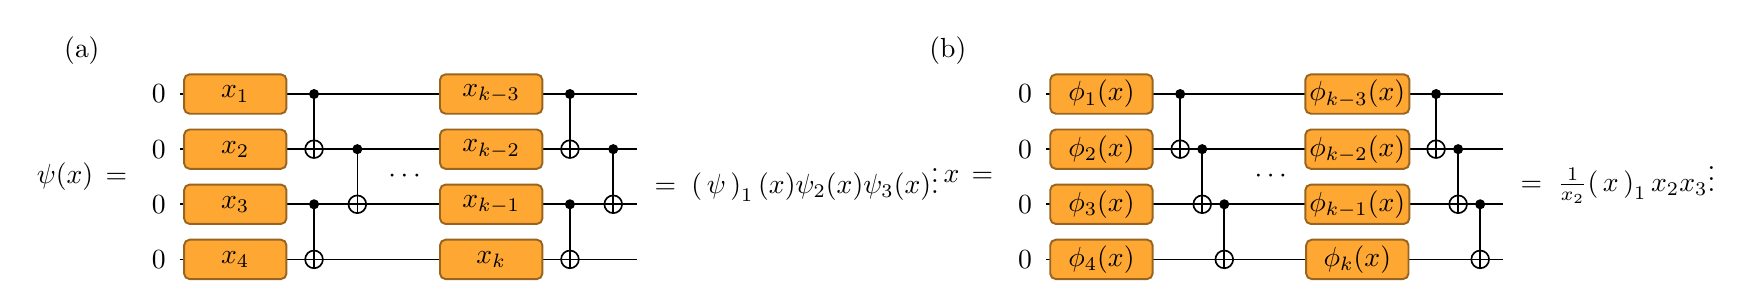
\begin{tikzpicture}[x=1cm,y=1cm]
% ============================== (a) angle encoding ==============================
\begin{scope}[xshift=0cm]
\node[font=\rmfamily] at (0.0, 0.55) {(a)};
\node[anchor=east] at (0.7,-1.05) {$\ket{\psi(x)}\,=$};
\foreach \i in {0,...,3}{
  \node at (0.98, -0.7*\i) {$\ket{0}$};
  \draw[qwire] (1.25, -0.7*\i) -- (7.05, -0.7*\i);
}
\node at (4.1,-1.05) {$\cdots$};
\foreach \i/\y in {1/0, 2/-0.7, 3/-1.4, 4/-2.1}{
  \node[bgate] at (1.95, \y) {$x_{\i}$};
}
\foreach \x/\ya/\yb in {2.95/0/-0.7, 2.95/-1.4/-2.1, 3.5/-0.7/-1.4}{
  \filldraw (\x,\ya) circle (1.6pt);
  \draw[qwire] (\x,\ya) -- (\x,\yb);
  \draw[qwire, fill=white] (\x,\yb) circle (3.2pt);
  \draw[qwire] (\x,{\yb-0.113}) -- (\x,{\yb+0.113});
  \draw[qwire] ({\x-0.113},\yb) -- ({\x+0.113},\yb);
}
\foreach \i/\y in {k-3/0, k-2/-0.7, k-1/-1.4, k/-2.1}{
  \node[bgate] at (5.2, \y) {$x_{\i}$};
}
\foreach \x/\ya/\yb in {6.2/0/-0.7, 6.2/-1.4/-2.1, 6.75/-0.7/-1.4}{
  \filldraw (\x,\ya) circle (1.6pt);
  \draw[qwire] (\x,\ya) -- (\x,\yb);
  \draw[qwire, fill=white] (\x,\yb) circle (3.2pt);
  \draw[qwire] (\x,{\yb-0.113}) -- (\x,{\yb+0.113});
  \draw[qwire] ({\x-0.113},\yb) -- ({\x+0.113},\yb);
}
\node[anchor=west] at (7.15,-1.05)
  {$=\;\begin{pmatrix} \psi_1(x)\\ \psi_2(x)\\ \psi_3(x)\\ \vdots \end{pmatrix}$};
\end{scope}
% ============================ (b) amplitude encoding ============================
\begin{scope}[xshift=11cm]
\node[font=\rmfamily] at (0.0, 0.55) {(b)};
\node[anchor=east] at (0.7,-1.05) {$\ket{x}\,=$};
\foreach \i in {0,...,3}{
  \node at (0.98, -0.7*\i) {$\ket{0}$};
  \draw[qwire] (1.25, -0.7*\i) -- (7.05, -0.7*\i);
}
\node at (4.1,-1.05) {$\cdots$};
\foreach \i/\y in {1/0, 2/-0.7, 3/-1.4, 4/-2.1}{
  \node[bgate] at (1.95, \y) {$\phi_{\i}(x)$};
}
\foreach \x/\ya/\yb in {2.95/0/-0.7, 3.23/-0.7/-1.4, 3.51/-1.4/-2.1}{
  \filldraw (\x,\ya) circle (1.6pt);
  \draw[qwire] (\x,\ya) -- (\x,\yb);
  \draw[qwire, fill=white] (\x,\yb) circle (3.2pt);
  \draw[qwire] (\x,{\yb-0.113}) -- (\x,{\yb+0.113});
  \draw[qwire] ({\x-0.113},\yb) -- ({\x+0.113},\yb);
}
\foreach \i/\y in {k-3/0, k-2/-0.7, k-1/-1.4, k/-2.1}{
  \node[bgate] at (5.2, \y) {$\phi_{\i}(x)$};
}
\foreach \x/\ya/\yb in {6.2/0/-0.7, 6.48/-0.7/-1.4, 6.76/-1.4/-2.1}{
  \filldraw (\x,\ya) circle (1.6pt);
  \draw[qwire] (\x,\ya) -- (\x,\yb);
  \draw[qwire, fill=white] (\x,\yb) circle (3.2pt);
  \draw[qwire] (\x,{\yb-0.113}) -- (\x,{\yb+0.113});
  \draw[qwire] ({\x-0.113},\yb) -- ({\x+0.113},\yb);
}
\node[anchor=west] at (7.15,-1.05)
  {$=\;\frac{1}{\lVert x\rVert_2}\!\begin{pmatrix} x_1\\ x_2\\ x_3\\ \vdots \end{pmatrix}$};
\end{scope}
\end{tikzpicture}%
}%
\endgroup
